\documentclass{beamer}
\mode<presentation>
{
  \usetheme{default}      % or try Darmstadt, Madrid, Warsaw, ...
  \usecolortheme{default} % or try albatross, beaver, crane, ...
  \usefonttheme{default}  % or try serif, structurebold, ...
  \setbeamertemplate{navigation symbols}{}
  \setbeamertemplate{caption}[numbered]
} 

\usepackage[english]{babel}
\usepackage[utf8x]{inputenc}
\usepackage[numbers]{natbib}

\usepackage{geometry}

\usepackage{subcaption}
\usepackage{amsmath}
\usepackage{mathtools}
\DeclarePairedDelimiter\abs{\lvert}{\rvert}%
\DeclarePairedDelimiter\norm{\lVert}{\rVert}%

\title[Hacking the Xgboost]{Coupon Challenge}
\author{Raul Sanchez-Vazquez}
\institute{}
\date{25 June 2018}

\begin{document}

\begin{frame}
  \titlepage
  
\end{frame}

\begin{frame}{The Problem}
	
	The problem:
	
	\begin{itemize}
		\item 	Create a recommender system for coupons.
	\end{itemize}

	This would be done in two stages:
		\begin{itemize}
			\item 	First, learn a model for classic top-n recommendation.
			\item 	Second, learn a binary classification model where the positive class correspond to actual purchase of the item.
		\end{itemize}
		
	Produce recommendation as:
	\begin{itemize}
		\item 	Produce candidate items (RecSys Model)
		\item 	Order by purchase probability (Positive probability score)
	\end{itemize}
\end{frame}
	
\begin{frame}{Analysis}
	
	We first built data profiling documents for:
	
	\begin{itemize}
		\item The item catalog.
		\item The user catalog.
		\item The user session log with purchase information.
	\end{itemize}
	
	We first noticed that the binary classification model would have to deal with class unbalance as shown on the plot below: 
	
	\begin{figure}
		\centering
		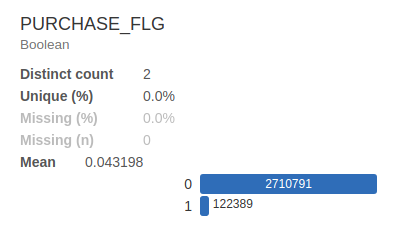
\includegraphics[width=0.7\linewidth]{../img/target}
		\caption{}
		\label{fig:target}
	\end{figure}
\end{frame}

\begin{frame}{Features}
	Item features:
	
\begin{itemize}
	\tiny
	\item item age promo
	\item item n views
	\item item n purchases
	\item item area
	\item item ken
	\item item small area
	\item item ken most buy
	\item item ken most buy2
	\item item large area most buy
	\item item large area most buy2
	\item item small area most buy
	\item item small area most buy2
	\item item buyers age mean
	\item item buyers age median
	\item item buyers age std
	\item item DISCOUNT PRICE percentage
	\item item price
	\item item purchase sex f
	\item item purchases sex m
\end{itemize}
\end{frame}

\begin{frame}{Features}
	User features:
	\begin{itemize}
			\tiny
		\item user same item n views
		\item user same item n purchases
		\item user last item large area name
		\item user last item ken name
		\item user last item small area name
		\item user purchases same item area
		\item user purchases same item ken name
		\item user purchases same item small area
		\item user AGE
		\item user SEX ID
	\end{itemize}
\end{frame}

\begin{frame}{Model Performance}

	Recsys on Test:
	\begin{itemize}
		\item P@10: 0.0018949648 
	\end{itemize}
	 
	Binary Classification on Test: 
		\begin{itemize}
			\item AUC:0.900254
		\end{itemize}
	
	\begin{figure}
	\centering
	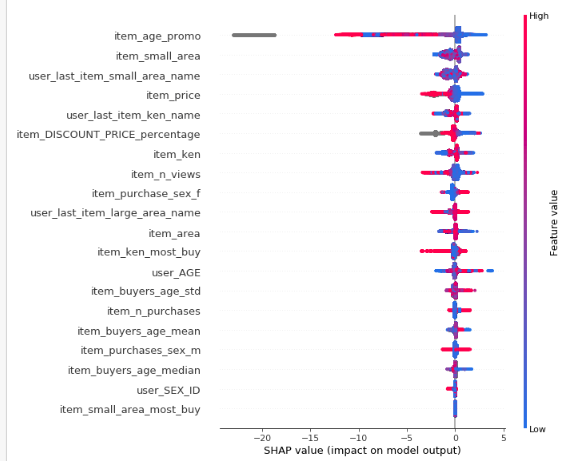
\includegraphics[width=0.7\linewidth]{../img/shap}
	\label{fig:shap}
	\end{figure}
\end{frame}

\begin{frame}{Model Performace}
	Hybrid recommender:

	\begin{itemize}
		\item P@10: 0.029458179905312992
	\end{itemize}
	
\end{frame}
	
\end{document}